\documentclass[10pt,letterpaper]{paper}

\usepackage{graphicx}
\usepackage{amsmath}
\usepackage{amssymb}
\usepackage{mathrsfs}
\usepackage{float}

\title{ HW1  }
\author{ Timothy Schwieg }
\date{ December 31 2017 }


\begin{document}

\maketitle

\section*{Question 1}

\subsection*{a}

\begin{figure}[H]
  \centering
  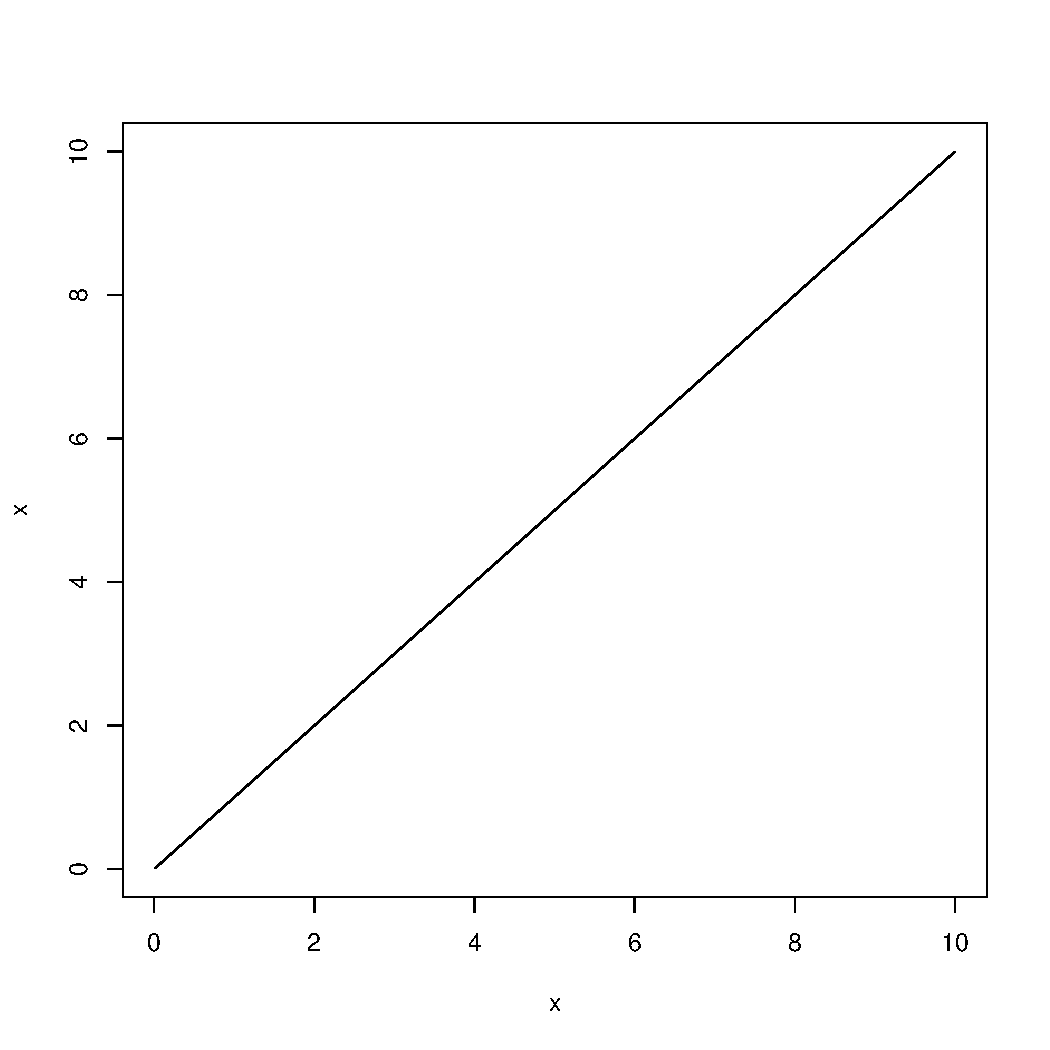
\includegraphics[scale=.3]{Question1a.pdf}
  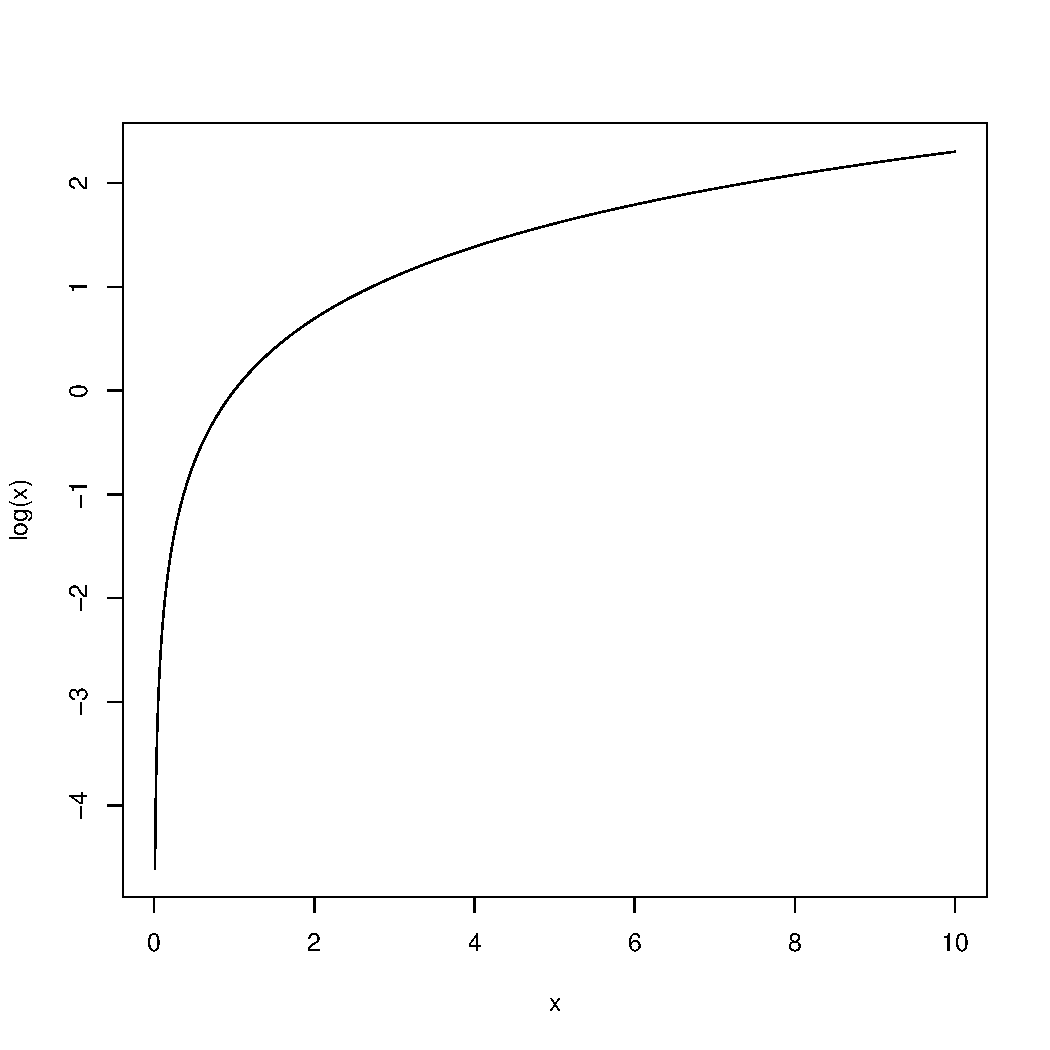
\includegraphics[scale=.3]{Question1b.pdf}
  \caption{\label{fig:label} }
\end{figure}

% \begin{figure}[H]
%   \centering
  
%   \caption{\label{fig:label} }
% \end{figure}

\begin{figure}[H]
  \centering
  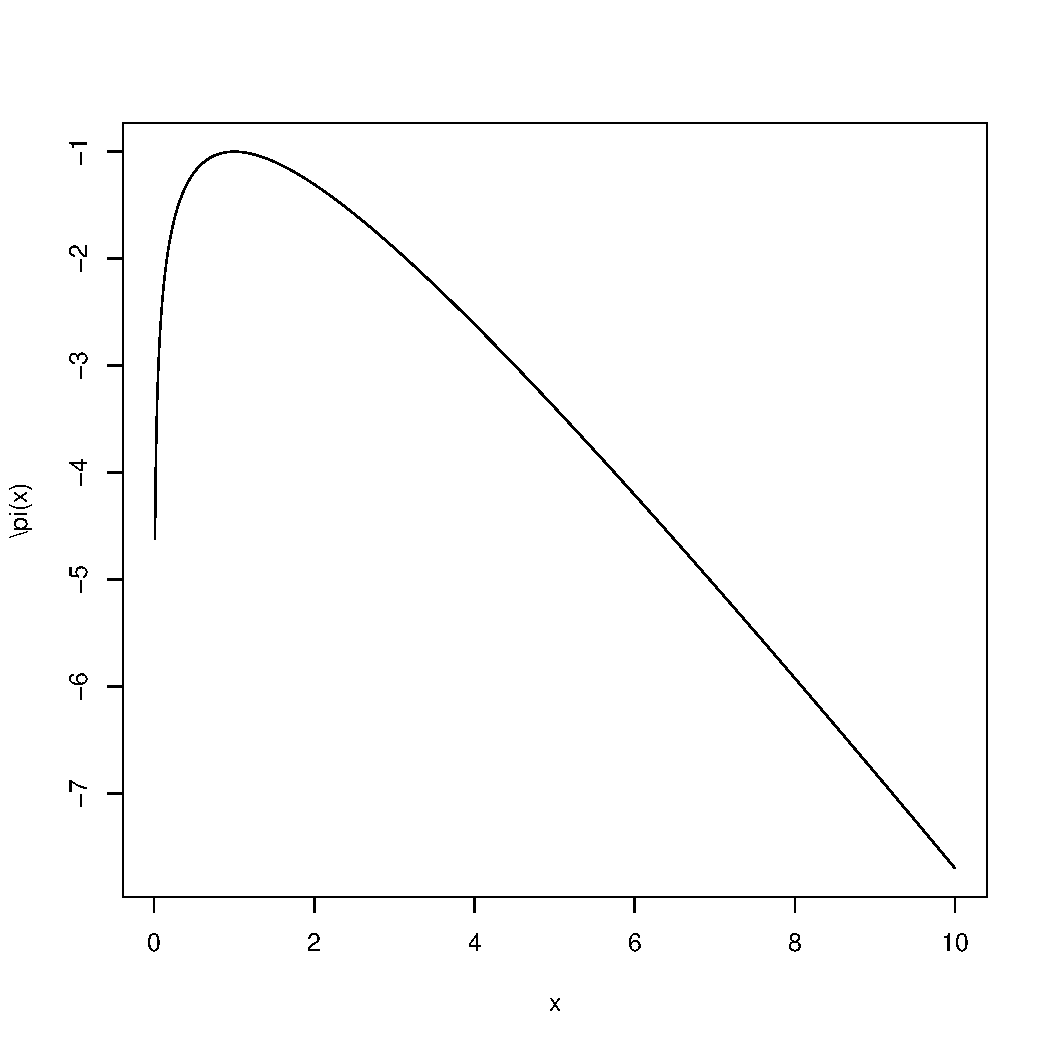
\includegraphics[scale=.25]{Question1c.pdf}
  \caption{\label{fig:label} }
\end{figure}


\subsection*{b}
\begin{align*}
  \frac{d}{dx} \pi(x) = \frac{1}{x} - 1 = 0\\
  \frac{1}{x} = 1\\
  1 = x
\end{align*}

\section*{Question 2}
\subsection*{a}
\begin{align*}
  \int_a^b y \frac{d}{dy} e^{ -y}dy = -y e^{ -y} + \int_a^b e^{-y}dy\\
  -y e^{ -y} - e^{ -y} \big |_a^b \\
  -b e^{ -b } - e^{ -b } + a e^{ -a } + e^{ -a }
\end{align*}
\subsection*{b}
\begin{align*}
  \lim_{x \to \infty } \int_0^x y \frac{d}{dy}e^{-y}dy &= \\
  \lim_{x \to \infty} -x e^{-x} - e^{-x} + 0e^0 + e^0 &= \\
  \lim_{x \to \infty} -x e^{-x} + 1 &= \\
  \lim_{x \to \infty} \frac{1}{e^{x}} + 1 &= 1
\end{align*}

\section*{Question 3}

\subsection*{a}

\begin{align*}
  \frac{dy}{dx}&=x\\
  dy &= xdx\\
  y &= \frac{1}{2}x^2 + C
\end{align*}

\subsection*{b}

\begin{align*}
  1 &= \frac{1}{2}0^2 + C\\
  1 &= C\\
  y &= \frac{1}{2}x^2 + 1
\end{align*}


\section*{Question 4}

\subsection*{CDF}

\begin{align*}
  F_V (v) &=
  \begin{cases}
    0 \text{ for } v < 0\\
    \int_0^v 1dv \text{ for } 0 \leq v \leq 1\\
    1 \text{ for } v > 1
  \end{cases}\\
  F_V(v) &=
  \begin{cases}
    0 \text{ for } v < 0\\
    v \text{ for } 0 \leq v \leq 1\\
    1 \text{ for } v > 1
  \end{cases}
\end{align*}

\subsection*{Mean}

\begin{align*}
  \mathbb{E}[X] &= \int_0^1 vdv\\
  \frac{1}{2}v^2 \big |_0^1 &= \frac{1}{2}
\end{align*}

\subsection*{Variance}
\begin{align*}
  Var(X) &= \mathbb{E}[X^2] - {\mathbb{E}[X]}^2\\
  \mathbb{E}[X^2] &= \int_0^1 v^2 dv = \frac{1}{3}v^3 \big |_0^1 = \frac{1}{3}\\
  Var(X) &= \frac{1}{3} - \frac{1}{4} = \frac{1}{12}
\end{align*}

\section*{Question 5}

\subsection*{a}
It is well understood that the distribution of a maximum of iid random variables
is given by:
\begin{align*}
  F_Z(z) = [F_V(z)]^N &=
  \begin{cases}
    0 \text{ for } z < 0\\
    [\int_0^z dv]^N \text{ for } 0 \leq z \leq 1\\
    1 \text{ for } z > 1
  \end{cases}\\
  F_Z(z) &=
  \begin{cases}
    0 \text{ for } z < 0 \\
    z^N \text{ for } 0 \le z \leq 1\\
    1 \text{ for } z > 1
  \end{cases}
\end{align*}
We may find the pdf of Z by taking the derivative of $F_Z(z)$ with respect to z.
\begin{align*}
  f_Z(z) = \frac{d}{dz} F_Z(z) =
  \begin{cases}
    0 \text{ for } z  \notin [0,1]\\
    Nz^{N-1} \text{ for } z \in [0,1]
  \end{cases}
\end{align*}

\subsection*{b}

\begin{align*}
  \mathbb{E}[X] = \int_0^1 N z^N = \frac{N}{N+1} z^{N+1} \big |_0^1 = \frac{N}{N+1}\\
  \mathbb{E}[X^2] = \int_0^1 N z^{N+1} = \frac{N}{N+2} z^{N+2} \big |_0^1 = \frac{N}{N+2}\\
  Var(X) = \mathbb{E}[X^2] - \mathbb{E}[X]^2 = \frac{N}{N+2}-(\frac{N}{N+1})^2 =\\
  \frac{N(N+1)^2}{(N+2)(N+1)^2} - \frac{N^2(N+2)}{(N+2)(N+1)^2} = \frac{N}{(N+2)(N+1)^2}
\end{align*}
\end{document}

